\subsection{Introduction}
Neural signals are firstly recorded as raw data. They exhibit two main components:
\begin{itemize}
    \item Local field potentials (LFPs) exist at low frequencies (\(0.1-300\,Hz\)).
          \begin{figure}[H]
              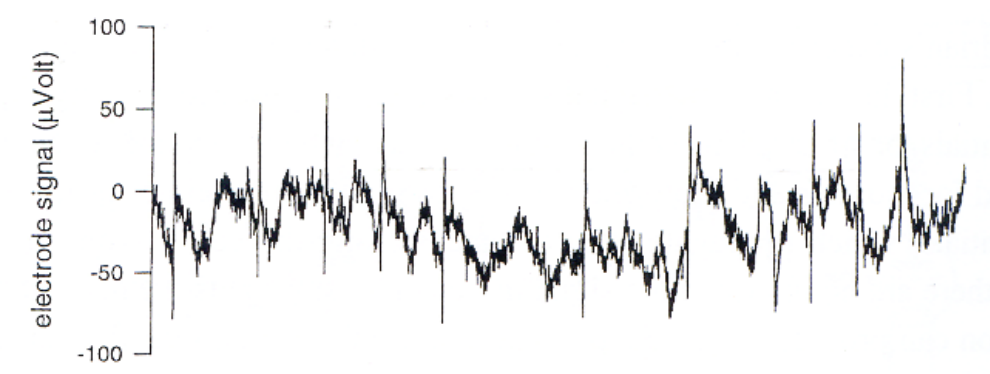
\includegraphics[scale=0.4]{2_1}
              \centering
          \end{figure}
    \item Spikes (MUA) exist at higher frequencies (\(300-3000\,Hz\)).
          \begin{figure}[H]
              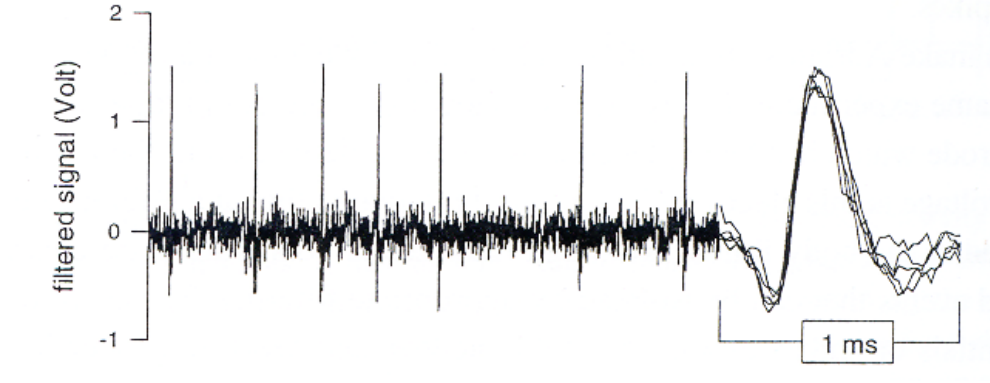
\includegraphics[scale=0.4]{2_2}
              \centering
          \end{figure}
\end{itemize}
The signal is obtained through extracellular recordings, then amplified and filtered. There are 3 possible
situations, according to the distance of the electrode tip from the neurons:
\begin{itemize}
    \item \(<50\,\mu{m}\): the SNR is good enough to distinguish the activity of a
          single neuron (single unit).
    \item \(50\sim150\,\mu{m}\): spikes are still detected, but the difference in their
          shape is masked by the noise (multi-unit activity or MUA).
    \item \(>150\,\mu{m}\): spikes cannot be detected and they contribute to the noise.
\end{itemize}
\begin{figure}[H]
    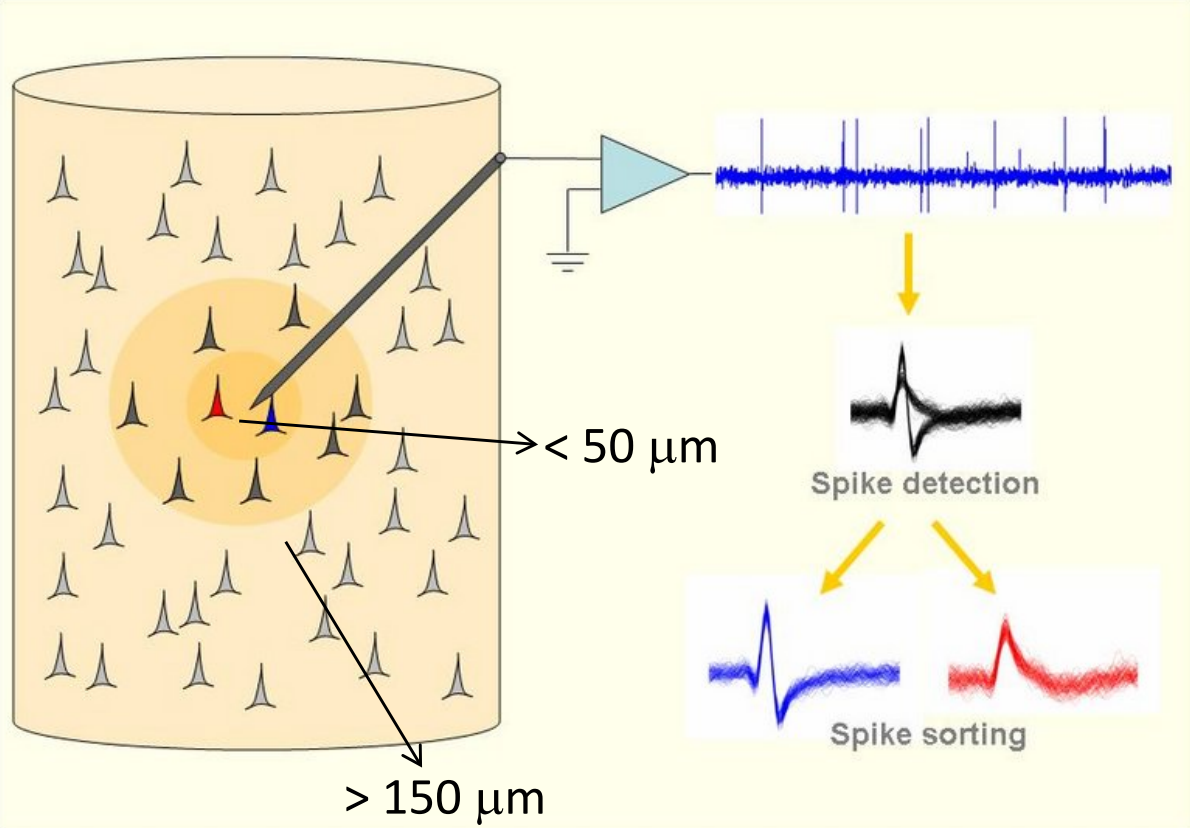
\includegraphics[scale=0.3]{2_3}
    \centering
\end{figure}
The electrophysiological signal, acquired from a single microelectrode is generally
characterized by two different patterns of activity:
\begin{itemize}
    \item \textbf{Spike}: single over-threshold signal representing the
          electrical activity of one or more neurons (1-3 cells).
    \item \textbf{Burst}: sequence of highly packed spikes often occurring simultaneously
          on several channels and giving rise to a phenomenon known as network burst.
\end{itemize}
The workflow commonly followed to preprocess this kind of data is:
\begin{figure}[H]
    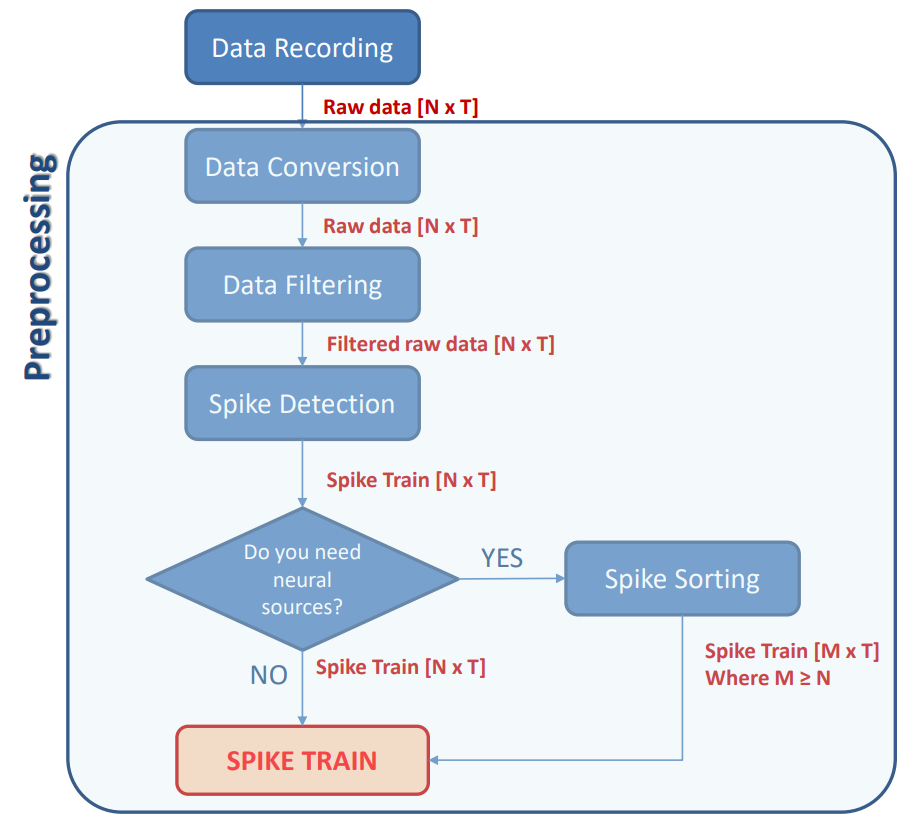
\includegraphics[scale=0.4]{2_4}
    \centering
\end{figure}
\begin{itemize}
    \item \textbf{Data recording:} raw data in the form of a matrix
    \item \textbf{Data conversion:} convert data to a form which is compatible with our system
    \item \textbf{Data filtering:} maintains the dimensionality but filters the data
    \item \textbf{Spike detection:} keeps always the same format (matrix)
    \item \textbf{Take a decision:} is it desirable to identify the individual sources of the signal?
          \begin{itemize}
              \item \textbf{No:} a multi-unit spike train is obtained
              \item \textbf{Yes:} Spike Sorting is performed to retrieve a spike train for
                    every individual source (single unit)
          \end{itemize}
\end{itemize}
Other than the preprocessing part, the other relevant part is the analysis itself, which is performed
by starting from the spike train:
\begin{figure}[H]
    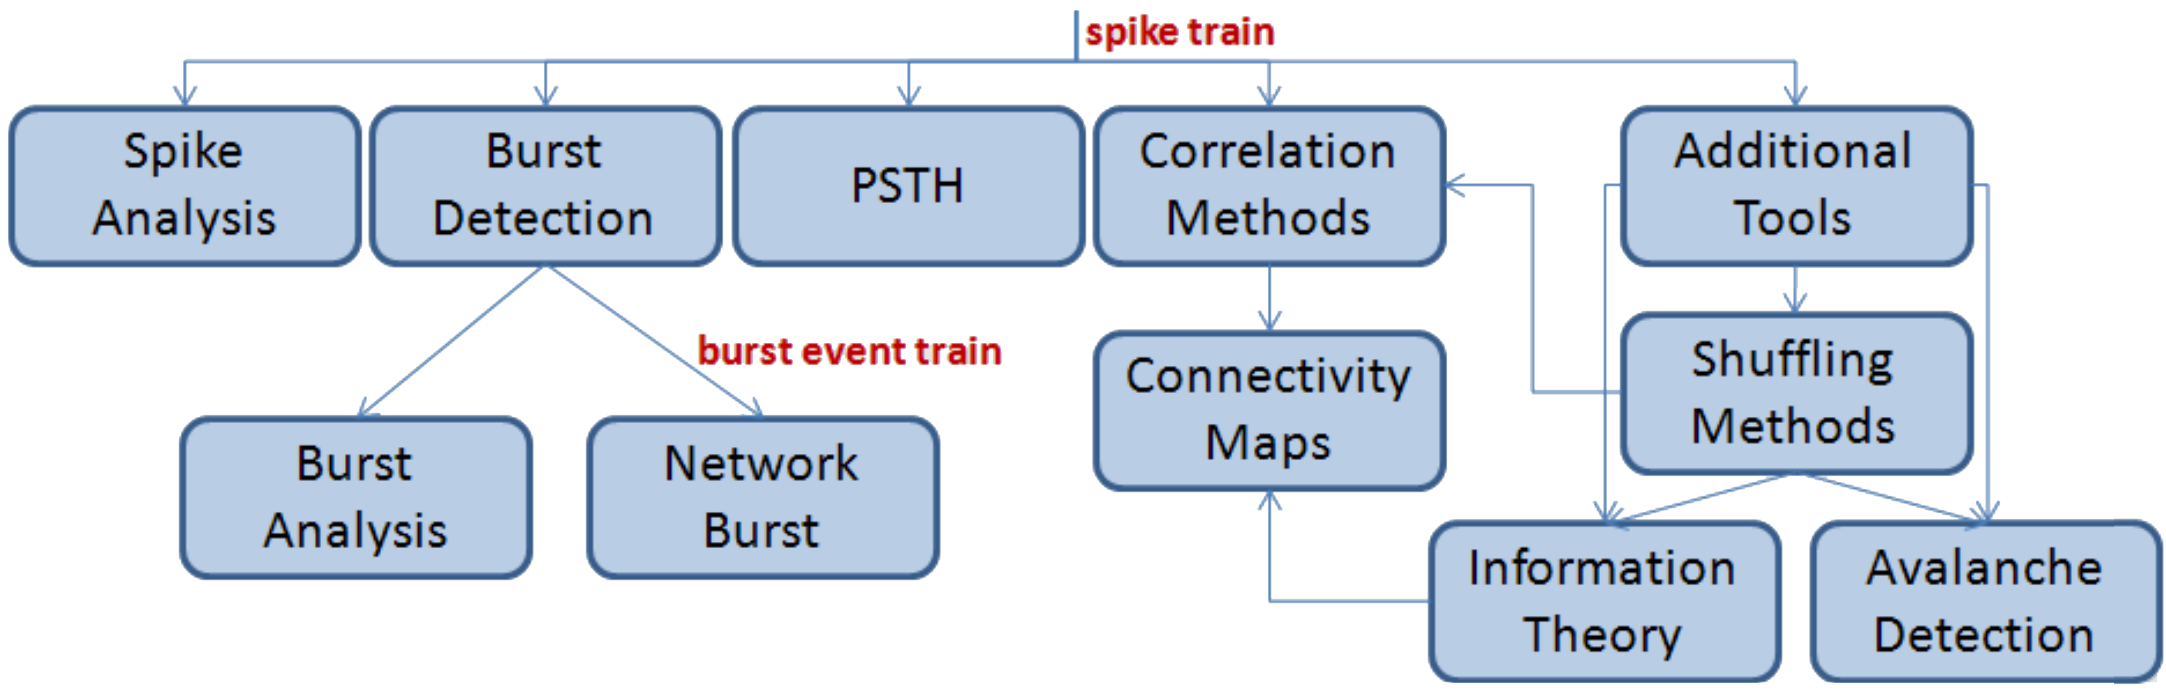
\includegraphics[scale=0.25]{2_5}
    \centering
\end{figure}
As already said, a spike train is a vector containing the positions of spikes with no information
regarding the amplitude (often normalized at \(1\)).
Let's recall the mathematically definition of a spike train:
\begin{itemize}
    \item Single-channel spike train:
          \begin{equation*}
              ST(t)=\sum_{s=1}^{N}\delta{(t-t_s)}
          \end{equation*}
    \item Multi-channel spike train:
          \begin{equation*}
              ST_j(t)=\sum_{s=1}^{N_j}\delta(t-t_s) \hspace{1cm} j=1,\dots,M
          \end{equation*}
\end{itemize}
\begin{figure}[H]
    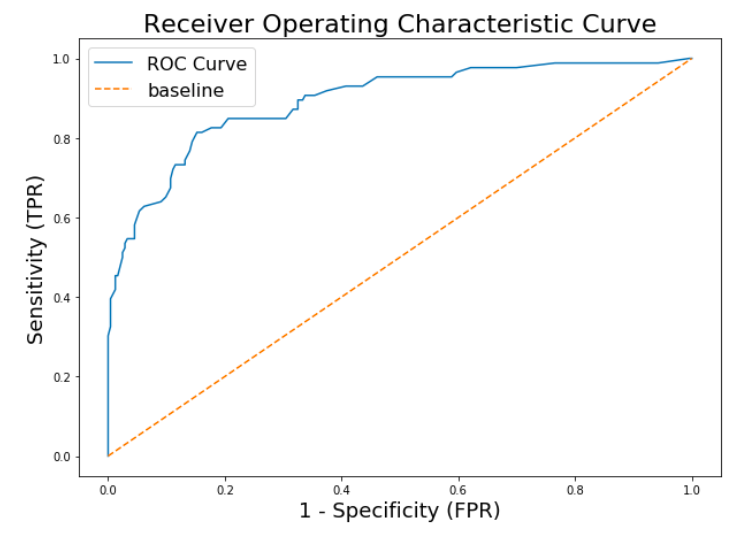
\includegraphics[scale=0.35]{2_6}
    \centering
\end{figure}
\textbf{Spike Detection:} it consists in recognizing the spikes within the raw data. It is the most
important step of the analysis, as it affects all the subsequent steps.\\
\textbf{Spike Sorting:} it is the process of associating each spike to a specific putative source
(classify spikes and individual sources).\\
When performing Spike Detection there are two main issues:
\begin{itemize}
    \item \textbf{Reliability} of the selected detection method
    \item \textbf{Precise position} of the detected peaks in the spike train
\end{itemize}

\subsection{Spike Detection algorithms}
So far, many algorithms have been developed but none of them has emerged as the best one yet.
They can be classified into 3 groups:
\begin{itemize}
    \item \textbf{Thresholding}: it is assumed that spikes peak-to-peak amplitude is larger than the noise level.
    \item \textbf{Energy operator}: non-linear energy operator accentuating high frequency content, i.e. spikes.
    \item \textbf{Template matching}: it is an approach based on the spike shape, involving Spike Sorting.
\end{itemize}
\subsubsection{Thresholding algorithms}
\paragraph{Simple Hard Threshold}
A \textbf{threshold} value is defined (either positive or negative). If the signal overcomes the threshold,
then a spike is detected. A \textbf{refractory period} (\(RP\)) between two peaks is employed to account for
subsequent samples overcoming the threshold after a spike detection.\\
Simple hard thresholding is characterized by a very simple logic and for this reason it is often employed in
commercial systems for data acquisition where the online detection of the spikes is required. This kind of
detection technique is often useful because it is quite fast, even if at the expenses of precision.
\begin{figure}[H]
    \centering
    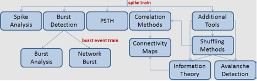
\includegraphics[scale=0.22]{2_7.png}
\end{figure}
\paragraph{Hard Threshold} Notice this algorithm is applied also to absolute-valued
signals. It involves 2 distinct main steps: application of a threshold and spike identification.\\
A time window denoted by \(T\) is applied to the signal, centering the window \(\frac{1}{3}T\) before the detected spike.
The length of \(T\) is to be carefully chosen, usually it is between \(1\) and \(3\,ms\), as it must minimize the likelihood
that more than one spike is captured in the window.\\
The threshold (\(Thr\)) can be defined in several ways:
\begin{itemize}
    \item \(Thr=n\sigma[V]\): \(n\) times the standard deviation \(\sigma\) of the basal signal noise.
    \item \(Thr=aP2P[V]\): fraction of the full amplitude (peak-to-peak) of the signal.
    \item \(Thr=n\sigma_N[V]\): \(n\) times the \(\sigma\) estimated from the
          Median Absolute Deviation (\(MAD\)), with \(MAD=median(|x-median(x)|)\) and \(\sigma_N=1.4826\cdot MAD\).
          A good value for \(n\) is \(4\).
\end{itemize}
\paragraph{Hard Threshold Local Maxima}
This method is very similar to the previous ones, but in this case the spike position is
associated to the local maxima (and not set at the time of the first sample overcoming the threshold).
\begin{figure}[H]
    \centering
    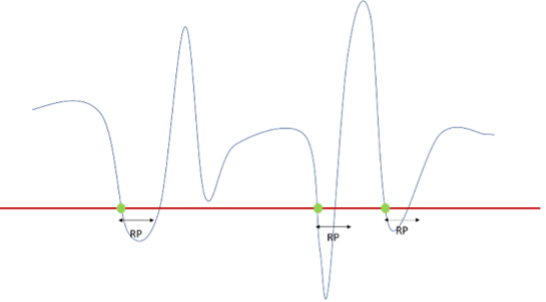
\includegraphics[scale=0.2]{2_8.png}
\end{figure}
\paragraph{Hard Threshold Differential Threshold}
A sliding window \(W\) is sized to contain at least one spike and is shifted over the signal.
The peak-to-peak threshold \(k\sigma\) is a multiple of the noise standard deviation (usually \(k=7\) or \(8\)).
A spike is detected in the \(i-\)th window when
\begin{equation*}
    [(max_i-min_i)\ge{k\sigma}]
\end{equation*}
with \(i=1,\dots,\frac{T}{W}\) and \(T\) being the entire duration of the signal.\\
This approach exhibits a major issue, which is related to undersampling if more spikes are found
in a single window (typically at the window borders).
\begin{figure}[H]
    \centering
    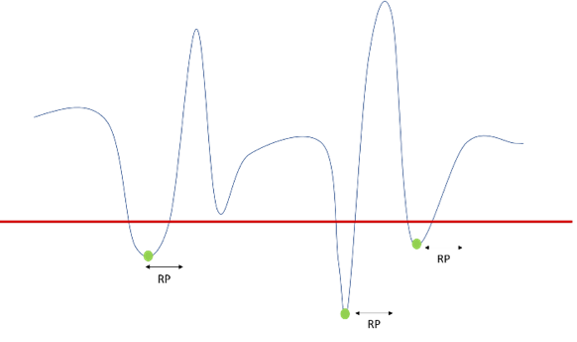
\includegraphics[scale=0.18]{2_9.png}
\end{figure}
\paragraph{Precision Timing Spike Detection (PTSD)}
This method solves the undersampling issue. \\ The operation of PTSD differs from the previous
algorithms in a variety of aspects: first and foremost, the presence of a differential threshold
instead of a unipolar one; moreover, in addition to \(RP\), there is also another time interval
called \textbf{Peak Lifetime Period} \(PLP\) (i.e. the maximum duration that a spike can have).
\begin{figure}[H]
    \centering
    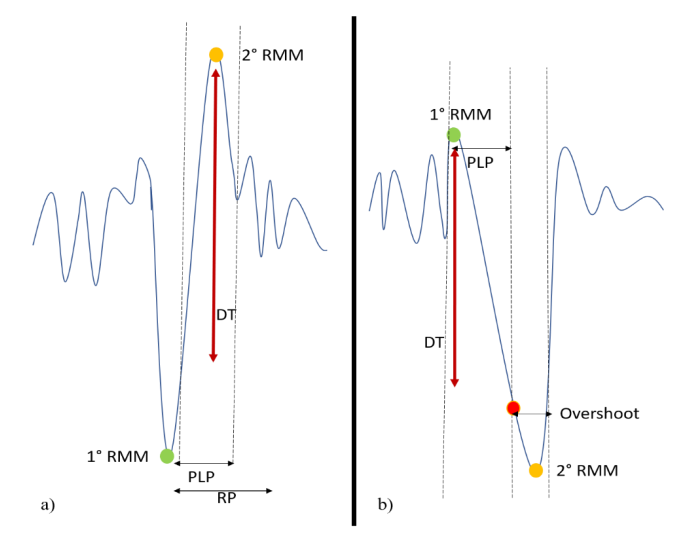
\includegraphics[scale=0.3]{2_10.png}
\end{figure}
Proceeding in order, the algorithm searches for a relative maximum/minimum (\(1^\circ\) \(RMM\),
Relative Maximum/Minimum): if it finds a maximum then it will search the signal for
the nearest minimum (\(2^\circ\) \(RMM\)) within the \(PLP\) window, while if it finds a minimum it will proceed
in the same way but looking for a maximum. If the difference between the first \(RMM\) and the second \(RMM\)
(i.e. the peak-to-peak amplitude of the spike), exceeds the Differential Threshold (\(DT\)),
then the spike is identified (\textit{Fig. a}). In case the second \(RMM\) falls at the end of the \(PLP\) window,
another time window called \textbf{overshoot} is used to find the correct peak value (\textit{Fig. b}). The \(DT\) is
always calculated as the standard deviation of the noise multiplied by a coefficient.\\
Of course, this algorithm can't be used in real time, because it needs future times, but it allows to detect also the
spikes passing through the boundaries of the considered window.
This technique is more demanding from the computational point of view, but it allows to detect
also the spikes passing through the boundaries of the considered window.
\subsubsection{Energy operator algorithms}
\paragraph{Signed Energy (SE)}
The SE algorithm is based on a moving window, whose width is set by the user,
which is used to scan the signal. For each time point, centered on the window width,
the energy is given by the sum of the squares of the voltage amplitudes within the
window, averaged by the window width:
\begin{equation*}
    SE(i)=\frac{1}{W}\sum_{j=i-\frac{W}{2}}^{j+\frac{W}{2}}V(j)^2
\end{equation*}
where \(V\) are the voltage amplitudes within the window and \(W\) is the window width.\\
The result is then multiplied by \(+1\) when the average amplitude of the raw signal is positive,
by \(-1\) when negative.\\
Since this algorithm has been implemented in the Offline Sorter commercial software,
we refer to it also as Offline Sorter Signed Energy (OSSE).
\paragraph{Nonlinear Energy Operator (NEO)}
The NEO algorithm is defined such that:
\begin{itemize}
    \item Constant voltage or zero \(\Rightarrow NE=0\)
    \item Waveform rapidly varying and a large amplitude \(\Rightarrow NE \text{ is maximum}\).
\end{itemize}
The \(NE\) of a signal \(x(n)\) is defined as:
\begin{align*}
    \psi[x(n)]=x^2(n)-x(n+1)\cdot x(n-1)
\end{align*}
The NEO is defined for each sample \(i\) and computed within a
window \(W\) centered in \(i\).\\
As a consequence, the NEO is large only when the signal is both high in power - i.e. \(x^2(n)\) is large -
and high in frequency - i.e. \(x(n)\) is large while \(x(n+1)\) and \(x(n-1)\) are small-.
Since a spike is characterized by localized high frequencies and an increase in instantaneous energy,
this method has an obvious advantage over methods that look only at an increase in signal energy or
amplitude without regarding the frequency.\\
The threshold is set to a scaled version of the mean of the NEO
\begin{align*}
    Thr=C\frac{1}{N}\sum_{n=1}^{N}\psi[x(n)]
\end{align*}
where \(N\) is the number of samples in the signal and \(C\) a scaling factor,
experimentally determined as \(C=8\).\\
If a smoothing window is applied after the NEO computing, the algorithm takes the name of smoothing NEO (SNEO).

\subsection{Assessing the Quality of a Spike Detection Method}
\subsubsection{Groundtruth}
In order to assess the performance of a Spike Detection algorithm, a groundtruth has to
be defined, such that several metrics of the tested algorithm can be computed.
A \textbf{groundtruth} is a collection of information (typically a dataset)
which is known to be true, opposed to information provided by inference.
There are 3 main types of groundtruths:
\begin{itemize}
    \item \textbf{Experimental groundtruth}: neurons are recorded into two distinct ways,
          extracellular and intracellular (or juxtacellular). Then a researcher uses the
          precise intracellular recordings (exhibting precise timing and localization) to find
          the same spikes into the extracellular signal.
    \item \textbf{Computational groundtruth}: data are synthetic and generated by a model
          reproducing the behaviour of a network of neurons under different conditions.\\
          In particular, this method enables the researcher to test the Spike Detection
          algorithms against datasets with different characteristics, such as different
          signal-to-noise ratios (SNR). This comparison using SNR can help to understand if
          the tested algorithm is reliable: if the peaks are identifiable also in bad
          conditions of SNR, then it is good.\\
          Notice that the SNR can be computed as the ratio of the mean of the peak to peak
          amplitude between all the spikes over 6 times the minimum noise standard deviation
          (evaluated in 10 different random intervals):
          \begin{equation*}
              SNR = \sqrt{\frac{\frac{1}{N}\sum_{i=1}^N(P2P_{up})_i}{6\sigma_{noise}}}
          \end{equation*}
    \item \textbf{Hybrid groundtruth}: natural and synthetic data are mixed.
          In particular, it is common to exploit manually detected and sorted spikes to be
          fed into computational models as input.
\end{itemize}
\subsubsection{Spike Detection Performance Evaluation}
Several distinct metrics can be taken into account when evaluating the performance of
a Spike Detection algorithm, in particular the most used ones are:
\begin{itemize}
    \item \textbf{Error count:}
          \begin{itemize}
              \item Type I error \(\Rightarrow\) False Positive (FP): incorrect
                    inclusion of noise, or spikes or other cells.
              \item Type II error \(\Rightarrow\) False Negative (FN): inability to
                    detect actual spikes.
          \end{itemize}
    \item \textbf{Position (mean) error:} the position of the
          detected spike is compared to the model one (mean error)
    \item \textbf{ROC curve}
\end{itemize}
\paragraph{Example} Hard Threshold algorithm errors\\
\begin{figure}[H]
    \centering
    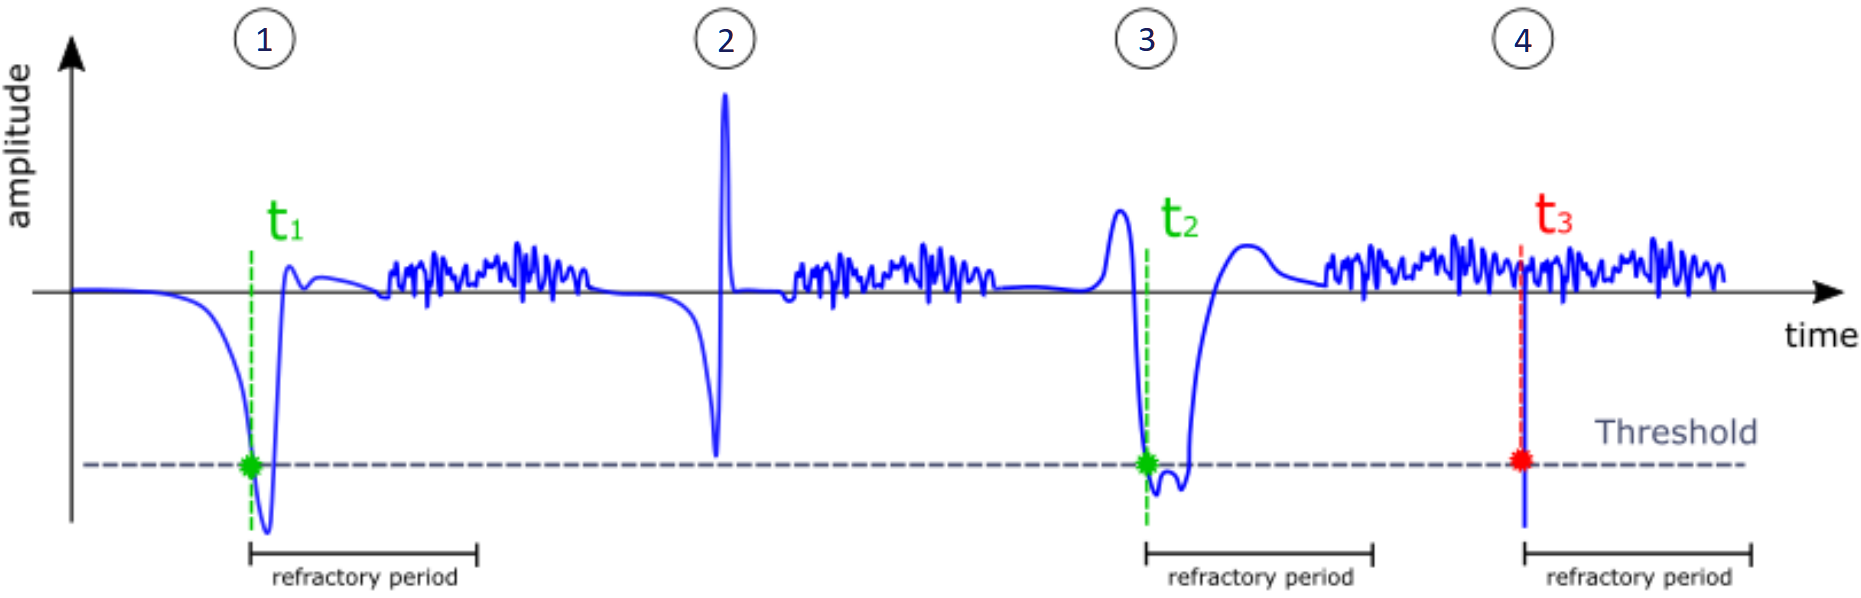
\includegraphics[scale=0.3]{2_11}
\end{figure}
\begin{enumerate}
    \item \textbf{True positive:} the algorithm detects all the samples above the threshold
          identifying as a spike position the first one, therefore the refractory period begins.
    \item \textbf{False negative:} if a spike occurs under the threshold, the algorithm
          misses it.
    \item \textbf{True positive:} the refractory period additionally helps to avoid the
          detection of double peaks which occasionally can occur in neural recordings.
    \item \textbf{False positive:} if some noise overcomes the threshold,
          a wrong spike is detected.
\end{enumerate}
A spike belonging to the spike train obtained from the tested algorithm is said to
have a \textbf{corresponding spike} in the groundtruth reference spike train if their
time distance is less than a defined threshold and no other spikes occur within
this time window.\\
Let's define the following variables:
\begin{itemize}
    \item \(NREF\): number of reference spikes (true spikes present in the groundtruth
          dataset)
    \item \(NDS\): number of detected spikes (spikes identified by the tested Spike
          Detection algorithm)
    \item \(NCS\): number of corresponding spikes (spikes correctly identified by
          the algorithm matching the groundtruth data)
\end{itemize}
The following expressions for False Positives and False Negatives can be derived:
\begin{align*}
    \text{\textbf{False Positives}}\Rightarrow FP=NDS-NCS
    \quad\quad\quad
    \text{\textbf{False Negatives}}\Rightarrow FN=NREF-NCS
\end{align*}
\begin{figure}[H]
    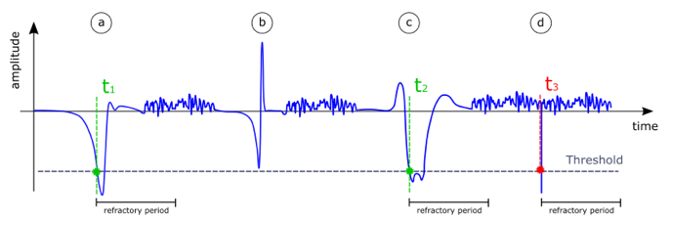
\includegraphics[scale=0.25]{2_12}
    \centering
\end{figure}
\paragraph{Receiver Operating Characteristics} The ROC curve is a well-known technique
for visualizing, organizing and selecting classifiers based on their performance.
In order to reduce the ROC performance to a single scalar indicator comprised between 0 and 1,
it is possible to calculate the Area Under the ROC Curve (AUC).\\
Notice that the ROC curve provides information regarding False Positives, but nothing
is said about False Negatives.
\paragraph{Confusion Matrix} This matrix is special type of contingecy matrix and
it allows to visualize the performance of an algorithm. Each row of the matrix
represents the instances in an actual class while each column represents the instances
in a predicted class (or vice versa). The confusion matrix term comes from the fact that
such a visualization allows to assess whether the system is confusing two classes.
\begin{figure}[H]
    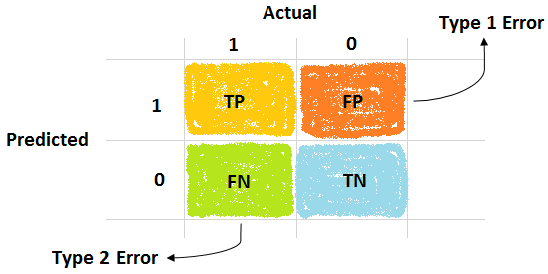
\includegraphics[scale=0.20]{2_13}
    \centering
\end{figure}
\paragraph{Other Metrics} Other useful metrics are introduced in the following.
\begin{align*}
    \begin{matrix}
        TP_{rate}   &  & \frac{Positives\,Correctly\,Classified}{Total\,Positives}=\frac{TP}{P}                 \\\\\\
        FP_{rate}   &  & \frac{Negatives\,Incorrectly\,Classified}{Total\,Negatives}=\frac{FP}{N}=1-Specificity \\\\\\
        Sensitivity &  & \frac{TP}{TP+FN}=\frac{TP}{P}=TP_{rate}                                                \\\\\\
        Specificity &  & \frac{TN}{TN+FP}=\frac{TN}{N}                                                          \\\\\\
        Accuracy    &  & \frac{TP+TN}{P+N}                                                                      \\\\\\
        Performance &  & \eta=\frac{TP}{FP+FN}                                                                  \\\\\\
        Efficiency  &  & \eta_2=\frac{\eta}{\eta+1}=\frac{TP}{TP+FN+FP}=\frac{TP}{P+FP}
    \end{matrix}
\end{align*}
